\chapter{Term Match Analysis}
\label{cha:analysis}
In this chapter, we mainly focus on recognizing the reasons that standard IR methods fail when the relevant patent documents are complete and in English. In fact, we will investigate what is wrong with respect to terms in both patent query and relevant documents. 
%%%%%%%%%%%%%%%%%%%%%%%%%%%%%%%%%%%%%%%%%%%%%%%%%%%%%%%%%%%%%%
\section{Term Mismatch}
\label{sec:termmismatch}
%\input{termmismatch}
%%%%%%%%%%%%%%%%%%%%%%%%%%%%%%%%%%%%%%%%%%%%%%%%%%%%%%%%%%%%%%
\begin{figure}[htpb]
%\begin{centering}
%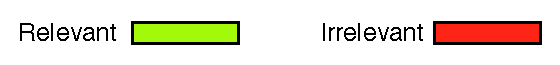
\includegraphics[width=9cm]{imgs/legend}
%\par\end{centering}

\begin{centering}
\subfigure[{Mean Average Precision.}]{\includegraphics[width=5cm]{figs/olap-fns-all.eps}}\subfigure[Recall.]{\includegraphics[width=5cm]{figs/olap-tps-all.eps}}\subfigure[Recall.]{\includegraphics[width=5cm]{figs/olap-fps-all.eps}}
\par\end{centering}

\protect\caption{System performance vs. the threshold $\tau$ for oracular query and oracular patent query.}
\label{fig:oracular}
\end{figure}
%%%%%%%%%%%%%%%%%%%%%%%%%%%%%%%%%%%%%%%%%%%%%%%%%%%%%%%%%%%%%%

%%%%%%%%%%%%%%%%%%%%%%%%%%%%%%%%%%%%%%%%%%%%%%%%%%%%%%%%%%%%%%
\section{Relevance Feedback}

\subsection{Discriminative Words}
\label{sec:discriminative}

\subsection{RF Optimal Query Formulation}
\label{sec:formulation}

\subsection{Query Reduction Using RF}

\section{Pseudo Relevance Feedback}

\subsection{PRF Query}
\subsection{Query Reduction Using RF}

\section{Noisy words}

\section{Section-based Analysis}

\subsection{Document Frequent Words}

\subsection{IPC Code Definition}

\section{Summary}
Same as the last chapter, summary what you discussed in this chapter and
be the bridge to next chapter.
